\documentclass[12pt,a4paper]{article}

\usepackage[a4paper,text={16.5cm,25.2cm},centering]{geometry}
\usepackage{lmodern}
\usepackage{amssymb,amsmath}
\usepackage{bm}
\usepackage{graphicx}
\usepackage{microtype}
\usepackage{hyperref}
\setlength{\parindent}{0pt}
\setlength{\parskip}{1.2ex}

\hypersetup
       {   pdfauthor = {  },
           pdftitle={  },
           colorlinks=TRUE,
           linkcolor=black,
           citecolor=blue,
           urlcolor=blue
       }




\usepackage{upquote}
\usepackage{listings}
\usepackage{xcolor}
\lstset{
    basicstyle=\ttfamily\footnotesize,
    upquote=true,
    breaklines=true,
    breakindent=0pt,
    keepspaces=true,
    showspaces=false,
    columns=fullflexible,
    showtabs=false,
    showstringspaces=false,
    escapeinside={(*@}{@*)},
    extendedchars=true,
}
\newcommand{\HLJLt}[1]{#1}
\newcommand{\HLJLw}[1]{#1}
\newcommand{\HLJLe}[1]{#1}
\newcommand{\HLJLeB}[1]{#1}
\newcommand{\HLJLo}[1]{#1}
\newcommand{\HLJLk}[1]{\textcolor[RGB]{148,91,176}{\textbf{#1}}}
\newcommand{\HLJLkc}[1]{\textcolor[RGB]{59,151,46}{\textit{#1}}}
\newcommand{\HLJLkd}[1]{\textcolor[RGB]{214,102,97}{\textit{#1}}}
\newcommand{\HLJLkn}[1]{\textcolor[RGB]{148,91,176}{\textbf{#1}}}
\newcommand{\HLJLkp}[1]{\textcolor[RGB]{148,91,176}{\textbf{#1}}}
\newcommand{\HLJLkr}[1]{\textcolor[RGB]{148,91,176}{\textbf{#1}}}
\newcommand{\HLJLkt}[1]{\textcolor[RGB]{148,91,176}{\textbf{#1}}}
\newcommand{\HLJLn}[1]{#1}
\newcommand{\HLJLna}[1]{#1}
\newcommand{\HLJLnb}[1]{#1}
\newcommand{\HLJLnbp}[1]{#1}
\newcommand{\HLJLnc}[1]{#1}
\newcommand{\HLJLncB}[1]{#1}
\newcommand{\HLJLnd}[1]{\textcolor[RGB]{214,102,97}{#1}}
\newcommand{\HLJLne}[1]{#1}
\newcommand{\HLJLneB}[1]{#1}
\newcommand{\HLJLnf}[1]{\textcolor[RGB]{66,102,213}{#1}}
\newcommand{\HLJLnfm}[1]{\textcolor[RGB]{66,102,213}{#1}}
\newcommand{\HLJLnp}[1]{#1}
\newcommand{\HLJLnl}[1]{#1}
\newcommand{\HLJLnn}[1]{#1}
\newcommand{\HLJLno}[1]{#1}
\newcommand{\HLJLnt}[1]{#1}
\newcommand{\HLJLnv}[1]{#1}
\newcommand{\HLJLnvc}[1]{#1}
\newcommand{\HLJLnvg}[1]{#1}
\newcommand{\HLJLnvi}[1]{#1}
\newcommand{\HLJLnvm}[1]{#1}
\newcommand{\HLJLl}[1]{#1}
\newcommand{\HLJLld}[1]{\textcolor[RGB]{148,91,176}{\textit{#1}}}
\newcommand{\HLJLs}[1]{\textcolor[RGB]{201,61,57}{#1}}
\newcommand{\HLJLsa}[1]{\textcolor[RGB]{201,61,57}{#1}}
\newcommand{\HLJLsb}[1]{\textcolor[RGB]{201,61,57}{#1}}
\newcommand{\HLJLsc}[1]{\textcolor[RGB]{201,61,57}{#1}}
\newcommand{\HLJLsd}[1]{\textcolor[RGB]{201,61,57}{#1}}
\newcommand{\HLJLsdB}[1]{\textcolor[RGB]{201,61,57}{#1}}
\newcommand{\HLJLsdC}[1]{\textcolor[RGB]{201,61,57}{#1}}
\newcommand{\HLJLse}[1]{\textcolor[RGB]{59,151,46}{#1}}
\newcommand{\HLJLsh}[1]{\textcolor[RGB]{201,61,57}{#1}}
\newcommand{\HLJLsi}[1]{#1}
\newcommand{\HLJLso}[1]{\textcolor[RGB]{201,61,57}{#1}}
\newcommand{\HLJLsr}[1]{\textcolor[RGB]{201,61,57}{#1}}
\newcommand{\HLJLss}[1]{\textcolor[RGB]{201,61,57}{#1}}
\newcommand{\HLJLssB}[1]{\textcolor[RGB]{201,61,57}{#1}}
\newcommand{\HLJLnB}[1]{\textcolor[RGB]{59,151,46}{#1}}
\newcommand{\HLJLnbB}[1]{\textcolor[RGB]{59,151,46}{#1}}
\newcommand{\HLJLnfB}[1]{\textcolor[RGB]{59,151,46}{#1}}
\newcommand{\HLJLnh}[1]{\textcolor[RGB]{59,151,46}{#1}}
\newcommand{\HLJLni}[1]{\textcolor[RGB]{59,151,46}{#1}}
\newcommand{\HLJLnil}[1]{\textcolor[RGB]{59,151,46}{#1}}
\newcommand{\HLJLnoB}[1]{\textcolor[RGB]{59,151,46}{#1}}
\newcommand{\HLJLoB}[1]{\textcolor[RGB]{102,102,102}{\textbf{#1}}}
\newcommand{\HLJLow}[1]{\textcolor[RGB]{102,102,102}{\textbf{#1}}}
\newcommand{\HLJLp}[1]{#1}
\newcommand{\HLJLc}[1]{\textcolor[RGB]{153,153,119}{\textit{#1}}}
\newcommand{\HLJLch}[1]{\textcolor[RGB]{153,153,119}{\textit{#1}}}
\newcommand{\HLJLcm}[1]{\textcolor[RGB]{153,153,119}{\textit{#1}}}
\newcommand{\HLJLcp}[1]{\textcolor[RGB]{153,153,119}{\textit{#1}}}
\newcommand{\HLJLcpB}[1]{\textcolor[RGB]{153,153,119}{\textit{#1}}}
\newcommand{\HLJLcs}[1]{\textcolor[RGB]{153,153,119}{\textit{#1}}}
\newcommand{\HLJLcsB}[1]{\textcolor[RGB]{153,153,119}{\textit{#1}}}
\newcommand{\HLJLg}[1]{#1}
\newcommand{\HLJLgd}[1]{#1}
\newcommand{\HLJLge}[1]{#1}
\newcommand{\HLJLgeB}[1]{#1}
\newcommand{\HLJLgh}[1]{#1}
\newcommand{\HLJLgi}[1]{#1}
\newcommand{\HLJLgo}[1]{#1}
\newcommand{\HLJLgp}[1]{#1}
\newcommand{\HLJLgs}[1]{#1}
\newcommand{\HLJLgsB}[1]{#1}
\newcommand{\HLJLgt}[1]{#1}


\begin{document}



\begin{lstlisting}
(*@\HLJLcs{{\#}Aleksa}@*) (*@\HLJLcs{Ćirković}@*)

(*@\HLJLcs{{\#}Naloga}@*) (*@\HLJLcs{je,}@*) (*@\HLJLcs{da}@*) (*@\HLJLcs{se}@*) (*@\HLJLcs{poveže}@*) (*@\HLJLcs{niz}@*) (*@\HLJLcs{točk}@*) (*@\HLJLcs{na}@*) (*@\HLJLcs{grafu}@*) (*@\HLJLcs{na}@*) (*@\HLJLcs{gladek}@*) (*@\HLJLcs{način.}@*) (*@\HLJLcs{Obstaja}@*) (*@\HLJLcs{več}@*) (*@\HLJLcs{točk,}@*) (*@\HLJLcs{vsaka}@*) (*@\HLJLcs{s}@*) (*@\HLJLcs{svojo}@*) (*@\HLJLcs{X}@*) (*@\HLJLcs{in}@*) (*@\HLJLcs{Y}@*) (*@\HLJLcs{vrednostjo,}@*) (*@\HLJLcs{in}@*) (*@\HLJLcs{je}@*) (*@\HLJLcs{potrebno}@*) (*@\HLJLcs{narisati}@*) (*@\HLJLcs{gladko}@*) (*@\HLJLcs{krivuljo,}@*) (*@\HLJLcs{ki}@*) (*@\HLJLcs{gre}@*) (*@\HLJLcs{skozi}@*) (*@\HLJLcs{vse}@*) (*@\HLJLcs{te}@*) (*@\HLJLcs{točke.}@*)

(*@\HLJLcs{{\#}Začne}@*) (*@\HLJLcs{se}@*) (*@\HLJLcs{s}@*) (*@\HLJLcs{seznamom}@*) (*@\HLJLcs{točk,}@*) (*@\HLJLcs{ki}@*) (*@\HLJLcs{jih}@*) (*@\HLJLcs{je}@*) (*@\HLJLcs{potrebno}@*) (*@\HLJLcs{povezati.}@*) (*@\HLJLcs{Vsaka}@*) (*@\HLJLcs{točka}@*) (*@\HLJLcs{ima}@*) (*@\HLJLcs{X}@*) (*@\HLJLcs{in}@*) (*@\HLJLcs{Y}@*) (*@\HLJLcs{vrednost.}@*)

(*@\HLJLcs{{\#}Za}@*) (*@\HLJLcs{povezovanje}@*) (*@\HLJLcs{teh}@*) (*@\HLJLcs{točk}@*) (*@\HLJLcs{z}@*) (*@\HLJLcs{gladko}@*) (*@\HLJLcs{krivuljo}@*) (*@\HLJLcs{uporablja}@*) (*@\HLJLcs{se}@*) (*@\HLJLcs{"{}Naravni}@*) (*@\HLJLcs{interpolacijski}@*) (*@\HLJLcs{kubični}@*) (*@\HLJLcs{zlepek"{}.}@*) (*@\HLJLcs{To}@*) (*@\HLJLcs{pomeni,}@*) (*@\HLJLcs{da}@*) (*@\HLJLcs{med}@*) (*@\HLJLcs{vsakim}@*) (*@\HLJLcs{parom}@*) (*@\HLJLcs{točk}@*) (*@\HLJLcs{narišete}@*) (*@\HLJLcs{mini-krivulje,}@*) (*@\HLJLcs{ki}@*) (*@\HLJLcs{se}@*) (*@\HLJLcs{lepo}@*) (*@\HLJLcs{prilegajo}@*) (*@\HLJLcs{skupaj}@*) (*@\HLJLcs{in}@*) (*@\HLJLcs{ustvarijo}@*) (*@\HLJLcs{eno}@*) (*@\HLJLcs{gladko}@*) (*@\HLJLcs{krivuljo.}@*)

(*@\HLJLcs{{\#}Na}@*) (*@\HLJLcs{koncu}@*) (*@\HLJLcs{se}@*) (*@\HLJLcs{nariše}@*) (*@\HLJLcs{ta}@*) (*@\HLJLcs{krivulja}@*) (*@\HLJLcs{na}@*) (*@\HLJLcs{grafu.}@*) (*@\HLJLcs{Za}@*) (*@\HLJLcs{boljšo}@*) (*@\HLJLcs{preglednost}@*) (*@\HLJLcs{tudi}@*) (*@\HLJLcs{so}@*) (*@\HLJLcs{označene}@*) (*@\HLJLcs{originalne}@*) (*@\HLJLcs{točke}@*) (*@\HLJLcs{in}@*) (*@\HLJLcs{uporabljene}@*) (*@\HLJLcs{različne}@*) (*@\HLJLcs{barve}@*) (*@\HLJLcs{za}@*) (*@\HLJLcs{prikaz}@*) (*@\HLJLcs{različnih}@*) (*@\HLJLcs{delov}@*) (*@\HLJLcs{krivulje.}@*)

(*@\HLJLcs{{\#}Struktura}@*) (*@\HLJLcs{Zlepek}@*) (*@\HLJLcs{je}@*) (*@\HLJLcs{osnova.}@*) (*@\HLJLcs{Hrani}@*) (*@\HLJLcs{vse}@*) (*@\HLJLcs{potrebne}@*) (*@\HLJLcs{informacije}@*) (*@\HLJLcs{o}@*) (*@\HLJLcs{interpolacijskih}@*) (*@\HLJLcs{točkah}@*) (*@\HLJLcs{(x}@*) (*@\HLJLcs{in}@*) (*@\HLJLcs{y}@*) (*@\HLJLcs{vrednosti)}@*) (*@\HLJLcs{ter}@*) (*@\HLJLcs{koeficiente}@*) (*@\HLJLcs{(a,}@*) (*@\HLJLcs{b,}@*) (*@\HLJLcs{c,}@*) (*@\HLJLcs{d),}@*) (*@\HLJLcs{ki}@*) (*@\HLJLcs{so}@*) (*@\HLJLcs{potrebni}@*) (*@\HLJLcs{za}@*) (*@\HLJLcs{izračun}@*) (*@\HLJLcs{kubičnih}@*) (*@\HLJLcs{zlepkov.}@*)

(*@\HLJLcs{{\#}Funkcija}@*) (*@\HLJLcs{interpoliraj}@*) (*@\HLJLcs{izračuna}@*) (*@\HLJLcs{koeficiente}@*) (*@\HLJLcs{za}@*) (*@\HLJLcs{kubični}@*) (*@\HLJLcs{zlepek}@*) (*@\HLJLcs{na}@*) (*@\HLJLcs{podlagi}@*) (*@\HLJLcs{danih}@*) (*@\HLJLcs{točk.}@*) (*@\HLJLcs{Uporablja}@*) (*@\HLJLcs{matriko}@*) (*@\HLJLcs{A}@*) (*@\HLJLcs{in}@*) (*@\HLJLcs{vektor}@*) (*@\HLJLcs{v}@*) (*@\HLJLcs{za}@*) (*@\HLJLcs{rešitev}@*) (*@\HLJLcs{sistema}@*) (*@\HLJLcs{enačb,}@*) (*@\HLJLcs{ki}@*) (*@\HLJLcs{določajo}@*) (*@\HLJLcs{koeficiente}@*) (*@\HLJLcs{zlepka.}@*) (*@\HLJLcs{Ti}@*) (*@\HLJLcs{koeficienti}@*) (*@\HLJLcs{so}@*) (*@\HLJLcs{ključni}@*) (*@\HLJLcs{za}@*) (*@\HLJLcs{risanje}@*) (*@\HLJLcs{gladke}@*) (*@\HLJLcs{krivulje}@*) (*@\HLJLcs{skozi}@*) (*@\HLJLcs{vse}@*) (*@\HLJLcs{dane}@*) (*@\HLJLcs{točke.}@*)

(*@\HLJLcs{{\#}Funkcija}@*) (*@\HLJLcs{vrednost}@*) (*@\HLJLcs{omogoča}@*) (*@\HLJLcs{izračun}@*) (*@\HLJLcs{vrednosti}@*) (*@\HLJLcs{interpolirane}@*) (*@\HLJLcs{krivulje}@*) (*@\HLJLcs{pri}@*) (*@\HLJLcs{kateri}@*) (*@\HLJLcs{koli}@*) (*@\HLJLcs{danem}@*) (*@\HLJLcs{x.}@*) (*@\HLJLcs{To}@*) (*@\HLJLcs{je}@*) (*@\HLJLcs{uporabno}@*) (*@\HLJLcs{za}@*) (*@\HLJLcs{preverjanje,}@*) (*@\HLJLcs{kako}@*) (*@\HLJLcs{dobro}@*) (*@\HLJLcs{krivulja}@*) (*@\HLJLcs{ustreza}@*) (*@\HLJLcs{podatkom}@*) (*@\HLJLcs{ali}@*) (*@\HLJLcs{za}@*) (*@\HLJLcs{napovedovanje}@*) (*@\HLJLcs{vrednosti}@*) (*@\HLJLcs{na}@*) (*@\HLJLcs{novih}@*) (*@\HLJLcs{točkah.}@*)

(*@\HLJLcs{{\#}Funkcija}@*) (*@\HLJLcs{plotDN}@*) (*@\HLJLcs{prikaže}@*) (*@\HLJLcs{graf,}@*) (*@\HLJLcs{ki}@*) (*@\HLJLcs{vizualno}@*) (*@\HLJLcs{predstavi}@*) (*@\HLJLcs{kako}@*) (*@\HLJLcs{krivulja}@*) (*@\HLJLcs{poteka}@*) (*@\HLJLcs{skozi}@*) (*@\HLJLcs{dane}@*) (*@\HLJLcs{točke.}@*) (*@\HLJLcs{Uporablja}@*) (*@\HLJLcs{se}@*) (*@\HLJLcs{za}@*) (*@\HLJLcs{preverjanje}@*) (*@\HLJLcs{pravilnosti}@*) (*@\HLJLcs{interpolacije}@*) (*@\HLJLcs{in}@*) (*@\HLJLcs{za}@*) (*@\HLJLcs{predstavitev}@*) (*@\HLJLcs{rezultatov.}@*) (*@\HLJLcs{Funkcija}@*) (*@\HLJLcs{menja}@*) (*@\HLJLcs{barve}@*) (*@\HLJLcs{med}@*) (*@\HLJLcs{segmenti}@*) (*@\HLJLcs{krivulje,}@*) (*@\HLJLcs{da}@*) (*@\HLJLcs{olajša}@*) (*@\HLJLcs{vizualno}@*) (*@\HLJLcs{analizo.}@*)

(*@\HLJLk{using}@*) (*@\HLJLn{Domaca01}@*)
(*@\HLJLk{using}@*) (*@\HLJLn{Plots}@*)

(*@\HLJLcs{{\#}}@*) (*@\HLJLcs{Nabor}@*) (*@\HLJLcs{točk,}@*) (*@\HLJLcs{za}@*) (*@\HLJLcs{interpolacijo}@*)
(*@\HLJLn{x{\_}tocke}@*) (*@\HLJLoB{=}@*) (*@\HLJLp{[}@*)(*@\HLJLnfB{1.0}@*)(*@\HLJLp{,}@*) (*@\HLJLnfB{2.0}@*)(*@\HLJLp{,}@*) (*@\HLJLnfB{3.0}@*)(*@\HLJLp{,}@*) (*@\HLJLnfB{4.0}@*)(*@\HLJLp{,}@*) (*@\HLJLnfB{5.0}@*)(*@\HLJLp{]}@*)
(*@\HLJLn{y{\_}tocke}@*) (*@\HLJLoB{=}@*) (*@\HLJLp{[}@*)(*@\HLJLnfB{1.0}@*)(*@\HLJLp{,}@*) (*@\HLJLnfB{4.0}@*)(*@\HLJLp{,}@*) (*@\HLJLnfB{9.0}@*)(*@\HLJLp{,}@*) (*@\HLJLnfB{16.0}@*)(*@\HLJLp{,}@*) (*@\HLJLnfB{25.0}@*)(*@\HLJLp{]}@*)

(*@\HLJLcs{{\#}}@*) (*@\HLJLcs{Funkcija}@*) (*@\HLJLcs{interpoliraj}@*) (*@\HLJLcs{za}@*) (*@\HLJLcs{izračun}@*) (*@\HLJLcs{koeficientov}@*)
(*@\HLJLn{zlepek}@*) (*@\HLJLoB{=}@*) (*@\HLJLn{Domaca01}@*)(*@\HLJLoB{.}@*)(*@\HLJLnf{interpoliraj}@*)(*@\HLJLp{(}@*)(*@\HLJLn{x{\_}tocke}@*)(*@\HLJLp{,}@*) (*@\HLJLn{y{\_}tocke}@*)(*@\HLJLp{)}@*)

(*@\HLJLcs{{\#}}@*) (*@\HLJLcs{Risanje}@*) (*@\HLJLcs{grafa}@*) (*@\HLJLcs{z}@*) (*@\HLJLcs{uporabo}@*) (*@\HLJLcs{funkcije}@*) (*@\HLJLcs{plotDN}@*)
(*@\HLJLn{Domaca01}@*)(*@\HLJLoB{.}@*)(*@\HLJLnf{plotDN}@*)(*@\HLJLp{(}@*)(*@\HLJLn{zlepek}@*)(*@\HLJLp{)}@*)

(*@\HLJLcs{{\#}}@*) (*@\HLJLcs{Prikaz}@*) (*@\HLJLcs{vrednost}@*) (*@\HLJLcs{krivulje}@*) (*@\HLJLcs{na}@*) (*@\HLJLcs{določeni}@*) (*@\HLJLcs{točki}@*)
(*@\HLJLcs{{\#}}@*) (*@\HLJLcs{Na}@*) (*@\HLJLcs{primer,}@*) (*@\HLJLcs{izračunati}@*) (*@\HLJLcs{vrednost}@*) (*@\HLJLcs{krivulje}@*) (*@\HLJLcs{pri}@*) (*@\HLJLcs{x}@*) (*@\HLJLcs{=}@*) (*@\HLJLcs{2.5}@*)
(*@\HLJLn{vrednost{\_}pri{\_}2{\_}5}@*) (*@\HLJLoB{=}@*) (*@\HLJLn{Domaca01}@*)(*@\HLJLoB{.}@*)(*@\HLJLnf{vrednost}@*)(*@\HLJLp{(}@*)(*@\HLJLn{zlepek}@*)(*@\HLJLp{,}@*) (*@\HLJLnfB{2.5}@*)(*@\HLJLp{)}@*)
(*@\HLJLnf{println}@*)(*@\HLJLp{(}@*)(*@\HLJLs{"{}Vrednost}@*) (*@\HLJLs{krivulje}@*) (*@\HLJLs{pri}@*) (*@\HLJLs{x}@*) (*@\HLJLs{=}@*) (*@\HLJLs{2.5}@*) (*@\HLJLs{je:}@*) (*@\HLJLsi{{\$}vrednost{\_}pri{\_}2{\_}5}@*)(*@\HLJLs{"{}}@*)(*@\HLJLp{)}@*)

(*@\HLJLcs{{\#}}@*) (*@\HLJLcs{Shranevanje}@*) (*@\HLJLcs{grafa}@*) (*@\HLJLcs{za}@*) (*@\HLJLcs{poročilo}@*)
(*@\HLJLnf{savefig}@*)(*@\HLJLp{(}@*)(*@\HLJLs{"{}interpolacijska{\_}krivulja.png"{}}@*)(*@\HLJLp{)}@*)
\end{lstlisting}

\begin{lstlisting}
Vrednost krivulje pri x = 2.5 je: 6.232142857142857
(*@{"{}}@*)C:(*@{{\textbackslash}}@*)(*@{{\textbackslash}}@*)Users(*@{{\textbackslash}}@*)(*@{{\textbackslash}}@*)Aki(*@{{\textbackslash}}@*)(*@{{\textbackslash}}@*)Files(*@{{\textbackslash}}@*)(*@{{\textbackslash}}@*)1MAG(*@{{\textbackslash}}@*)(*@{{\textbackslash}}@*)NM(*@{{\textbackslash}}@*)(*@{{\textbackslash}}@*)nummat-2324(*@{{\textbackslash}}@*)(*@{{\textbackslash}}@*)DomNal(*@{{\textbackslash}}@*)(*@{{\textbackslash}}@*)interpolacijska(*@{{\_}}@*)kriv
ulja.png(*@{"{}}@*)
\end{lstlisting}

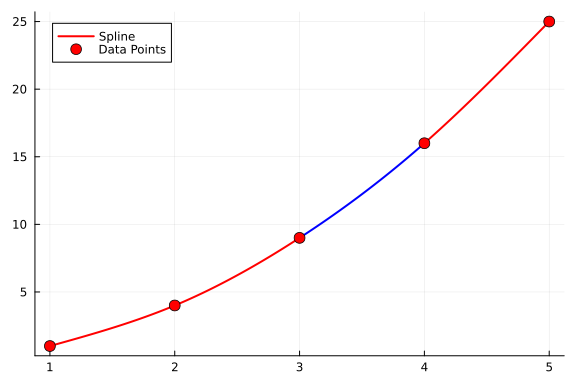
\includegraphics[width=\linewidth]{jl_sCze9i/demo_0_1.pdf}


\end{document}
